\textline[t]{\Large{6}}{\scshape{К\,В\,А\,Н\,Т $\cdot$ 1998 /\:\textnumero3}}

\begin{multicols}{3} \small
малый угол
\\

$\alpha \simeq 2\rho\textit{v}^2S_x\slash(mg) \simeq 5\cdot10^{-6}рад \simeq 1''$.
\\

Однако за сутки спутник совершает более 16 оборотов, и, спускаясь все ниже и ниже, где плотность атмосферы очень резко возрастает, он все круче и круче «зарывается» в атмосферу Земли. На высоте 150 км, где $\rho\simeq 4\cdot10^{-9}$ кг/м$^3$, за один виток этот же спутник снизится на 20 км! Еще один-два витка, и спутник попадает в столь плотную воздушную среду, что не может завершить очередной виток и, вместо того чтобы двигаться по спирали, начинает падать почти отвесно, испытывая при этом большие механические нагрузки и тепловой удар. Наступает неминуемый конец его орбитального путешествия. Легкие, пустотелые спутники падают раньше, сходят с орбиты на больших высотах, тяжелым удается вращаться вокруг Земли ближе к ее поверхности.

\begin{Figure}
\centering
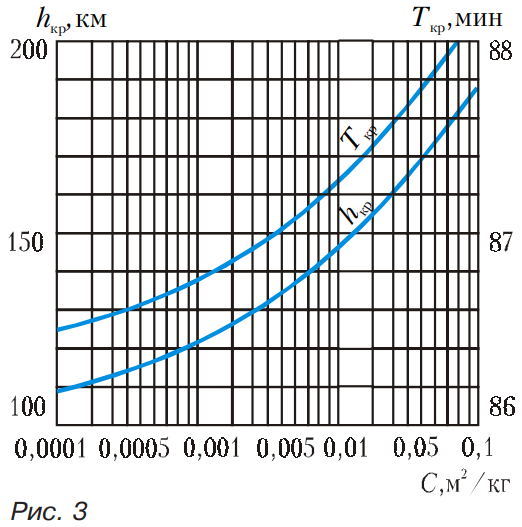
\includegraphics[width=\textwidth]{pic.jpg}
\end{Figure}

На рисунке 3 показано, как критическая высота и, соответственно, критическое время обращения спутника вокруг Земли зависят от его баллистического параметра $C$. Например, корабль «Восток», на котором летал Юрий Гагарин, имел массу 2,4 т и диаметр 2,3 м, т.е. баллистический коэффициент корабля был равен $C=1,7\cdot10^{-3}$ м$^2\cdot$кг$^{-1}$. Как видно из графика, критическая высота полета составляет $h_\textit{кр}\simeq130$ км, а критическое время обращения — $T_\textit{кр}\simeq 86$ мин $54$ с. Спутник, о котором шла речь выше, имеет примерно такое же отношение $S_x/m$, как корабль «Восток», и близкие критические параметры орбиты, в частности — критическая высота полета спутника составляет около 125 км. Заметим, что для ледяного шарика диаметром 1 см критическая высота превышает 200 км, а для меньших частиц она еще больше! Атмосфера и Земля работают как пылесос, исправно удаляя мелкий космический мусор с околоземных орбит. 

И еще одно. Когда спутник, спускаясь, приближается к критической высоте, сила сопротивления среды все еще не так велика по сравнению с силой тяжести спутника. Она примерно во столько же раз меньше нее, во сколько эффективная толщина атмосферы меныше радиуса Земли, умноженного на 4$\pi$ (см. формулу (6)), т.е. составляет примерно десятитысячную часть от силы тяжести. Мало? Но этого уже достаточно, чтобы спутник очень скоро исчез.

\textbf{Пример 3.} \textit{Время жизни спутника в орбитальном полете.}

Протяженный атмосферный «хвост» укорачивает жизнь спутника. Формулы, которые есть в нашей статье, позволяют сделать оценку времени жизни спутника, если известны начальная высота полета и высотный профиль плотности атмосферы. Хотя проведение точных расчетов — достаточно трудоемкая операция, в приближенных оценках можно учитывать, что основное время жизни спутника связано с нахождением его на самых верхних орбитах, тде плотность воздуха наименьшая. Результаты оценок зависят от типа. спутника, точнее — от его баллистического параметра $C$. Не будем здесь рассматривать само решение этой задачи (тем более что один из ее вариантов опубликован в журнале «Квант» №2 за 1996 год в статье «V Международная олимпиада «Интеллектуальный марафон» — см. задачу 3 по физике), а только приведем в форме таблицы результаты оценочных величин времени жизни обычных исследовательских спутников на орбитах с разными начальными высотами полета:
\begin{center}
\begin{tabular}{|l|l|}
    \hline
    Высота полета (км) & Время жизни \\
    \hline
    150 & 1 сутки \\
    190 & 2 суток \\
    210 & 1 неделя \\
    230 & 1 месяц \\
    400 & 1 год \\
    500 & 10 лет \\
    650 & 100 лет \\
    850 & 1000 лет \\
    1300 & 10 тыс. лет \\
    2000 & 100 тыс. лет \\
    \hline
\end{tabular}
\end{center}

Эта таблица иллюстрирует, прежде всего, сколь резко убывает плотность воздуха на больших высотах при удалении от земной поверхности. Таблица помогает также ответить на вопрос, почему спутник, на борту которого устанавливается аппаратура, рассчитанная на многолетнюю программу исследований, выводится на орбиту высотой не менее 500 км.
В заключение предлагаем несколько задач и вопросов для самостоятельной работы.

\textbf{Упражнения}

\begin{enumerate}[label=\textbf{\arabic*}.]
    \item Первые запуски спутников продемонстрировали нечто любопытное. При выводе на орбиту и отделении спутника от последней ступени ракеты-носителя ракета с уже выключенными двигателями обгоняла спутник и вырывалась вперед. Как объяснить это явление? Можно считать, что в момент отделения скорости ракеты и спутника одинаковые.
    \item Объясните, почему из-за торможения спутника в верхних слоях атмосферы его первоначально эллиптическая орбита стремится стать круговой.
    \item Покажите, что если бы плотность воздуха убывала с высотой по закону $\rho \sim R^{-1/2}$, где $R$ — расстояние от центра планеты, то скорость уменьшения радиуса орбиты спутника была бы постоянной.
    \item Спутник вращается по окружности в поле планеты с разреженной атмосферой. Предположим, что сила притяжения к планете подчиняется закону $F \sim R^{-n}$, где $n$ -- произвольное положительное число (случай $n$\,=\,$2$, как известно, соответствует ньютоновскому тяготению). При каких и возможен аэродинамический парадокс спутника?
    \item Зависит ли торможение спутника на больших высотах от температуры воздуха?
    \item Допустим, что в результате сильного нагрева Земли вся вода в океанах испарилась, а планета покрылась плотной и горячей атмосферой из водяного пара. Как это скажется на движении существующих ныне искусственных спутников Земли и ее естественного спутника Луны?
\end{enumerate}

\end{multicols}
